\documentclass[final,hyperref={pdfpagelabels=false}]{beamer}
\usepackage{grffile}
\mode<presentation>{\usetheme{kaldi1}}
\usepackage[english]{babel}
\usepackage[latin1]{inputenc}
\usepackage{amsmath,amsthm, amssymb, latexsym, listings}
%\usepackage{times}\usefonttheme{professionalfonts}  % obsolete
%\usefonttheme[onlymath]{serif}
\boldmath
\usepackage[orientation=landscape,size=a0,scale=1.4,debug]{beamerposter}
% change list indention level
% \setdefaultleftmargin{3em}{}{}{}{}{}


%\usepackage{snapshot} % will write a .dep file with all dependencies, allows for easy bundling

\usepackage{array,booktabs,tabularx}
\newcolumntype{Z}{>{\centering\arraybackslash}X} % centered tabularx columns
\newcommand{\pphantom}{\textcolor{kaldiblack}} % phantom introduces a vertical space in p formatted table columns??!!

\listfiles

%%%%%%%%%%%%%%%%%%%%%%%%%%%%%%%%%%%%%%%%%%%%%%%%%%%%%%%%%%%%%%%%%%%%%%%%%%%%%%%%%%%%%%
\graphicspath{{figures/}}
 
\title{\huge The Kaldi Speech Recognition Toolkit}
\author{{Daniel Povey}$^1$, {Arnab Ghoshal}$^{2,3}$,
  {Gilles Boulianne}$^4$, {Luk\'{a}\v{s} Burget}$^{5,6}$, {Ond\v{r}ej 
    Glembek}$^5$, {Nagendra Goel}$^6$, \\
  {Mirko Hannemann}$^5$, 
  {Petr Motl\'{i}\v{c}ek}$^8$, {Yanmin Qian}$^9$, {Petr Schwarz}$^5$, 
  {Jan Silovsk\'{y}}$^{10}$, {Georg Stemmer}$^{11}$, {Karel Vesel\'{y}}$^5$}
\institute[]{   $^1$\,Microsoft Research, USA;
   $^2$\,University of Edinburgh, UK;
   $^3$\,Saarland University, Germany;
   $^4$\,Centre de Recherche Informatique de Montr\'{e}al, Canada; 
   $^5$\,Brno University of Technology, Czech Republic;
   $^6$\,SRI International, USA;
   $^7$\,Go-Vivace Inc., USA; $^8$\,IDIAP Research Institute, Switzerland; 
   $^9$\,Tsinghua University, China;
   $^{10}$\,Technical University of Liberec, Czech Republic; 
   $^{11}$\,University of Erlangen-Nuremberg, Germany
}
\date[]{}

%%%%%%%%%%%%%%%%%%%%%%%%%%%%%%%%%%%%%%%%%%%%%%%%%%%%%%%%%%%%%%%%%%%%%%%%%%%%%%%%%%%%%%
\newlength{\columnheight}
\setlength{\columnheight}{65cm}


%%%%%%%%%%%%%%%%%%%%%%%%%%%%%%%%%%%%%%%%%%%%%%%%%%%%%%%%%%%%%%%%%%%%%%%%%%%%%%%%%%%%%%
\begin{document}
\begin{frame}[fragile]
  \begin{columns}
    % ---------------------------------------------------------%
    % Set up a column 
    \begin{column}{.33\textwidth}
      \begin{beamercolorbox}[center,wd=\textwidth]{postercolumn}
        \begin{minipage}[T]{.95\textwidth}  % tweaks the width, makes a new \textwidth
          \parbox[t][\columnheight]{\textwidth}{ % must be some better way to set the the height, width and textwidth simultaneously
            % Since all columns are the same length, it is all nice and tidy.  You have to get the height empirically
            % ---------------------------------------------------------%
            % fill each column with content            
            \begin{block}{Features of Kaldi}
              \begin{columns}
                \begin{column}{.44\textwidth}
              \begin{itemize}
              \item Integration with Finite State Transducers
              \item Extensive linear algebra support
              \item Extensible design
              \item Open license
              \item Complete recipes
              \item Thorough testing
              \end{itemize}
                \end{column}
                \begin{column}{.55\textwidth}
                  \centering
                  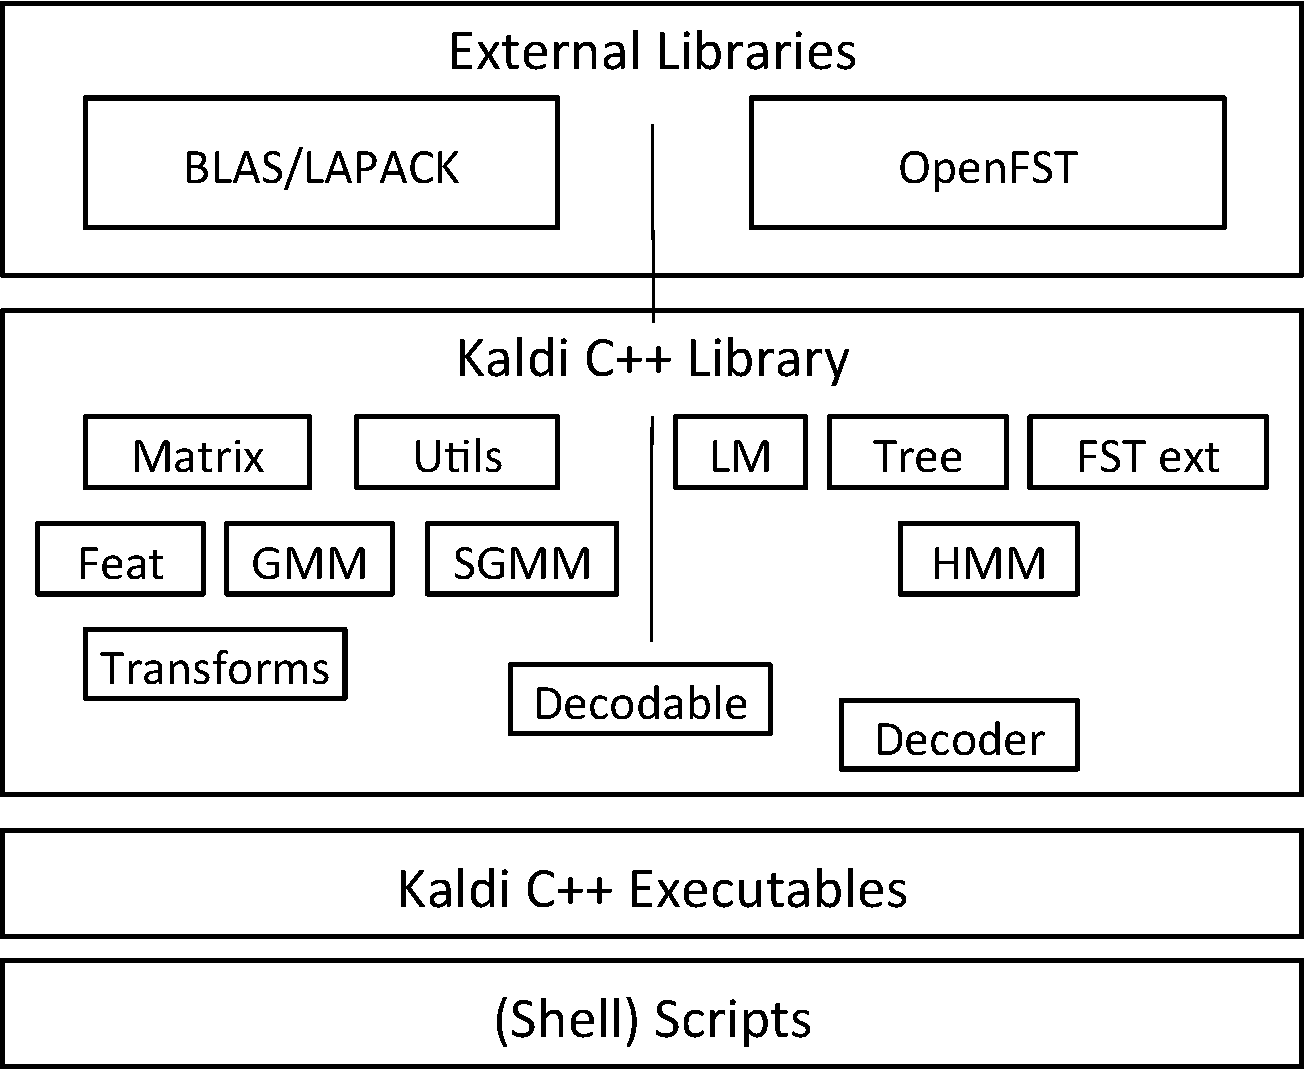
\includegraphics[width=0.85\linewidth]{figures/kaldi-lib.pdf}
                \end{column}
              \end{columns}
              \vskip-1ex
            \end{block}
            \vfill
            \begin{block}{Standard ASR techniques supported in Kaldi}
              \begin{itemize}
              \item Acoustic front-end supports MFCC and PLP features, with 
                cepstral mean and variance normalization, LDA, STC/MLLT, HLDA,
                VTLN, etc.
              \item HMM/GMM acoustic models 
              \item No language modeling code, but support converting ARPA 
                format LMs to FSTSs.
              \end{itemize}
            \end{block}
            \vfill
            \begin{block}{Features unique to Kaldi}
              \begin{itemize}
              \item SGMM acoustic models
              \item Exponential transform
              \end{itemize}
            \end{block}
          }
        \end{minipage}
      \end{beamercolorbox}
    \end{column}
    % ---------------------------------------------------------%
    % end the column

    % ---------------------------------------------------------%
    % Set up a column 
    \begin{column}{.33\textwidth}
      \begin{beamercolorbox}[center,wd=\textwidth]{postercolumn}
        \begin{minipage}[T]{.95\textwidth} % tweaks the width, makes a new \textwidth
          \parbox[t][\columnheight]{\textwidth}{ % must be some better way to set the the height, width and textwidth simultaneously
            % Since all columns are the same length, it is all nice and tidy.  You have to get the height empirically
            % ---------------------------------------------------------%
            % fill each column with content
            
            \begin{block}{The Kaldi Decoder}
% \begin{verbatim}
% class DecodableInterface {
%  public:
%   virtual float LogLikelihood(int frame, int index) = 0;
%   virtual bool IsLastFrame(int frame) = 0;
%   virtual int NumIndices() = 0;
%   virtual ~DecodableInterface() {}
% };
% \end{verbatim}
            \end{block}
          }
        \end{minipage}
      \end{beamercolorbox}
    \end{column}
    % ---------------------------------------------------------%
    % end the column

    % ---------------------------------------------------------%
    % Set up a column 
    \begin{column}{.33\textwidth}
      \begin{beamercolorbox}[center,wd=\textwidth]{postercolumn}
        \begin{minipage}[T]{.95\textwidth} % tweaks the width, makes a new \textwidth
          \parbox[t][\columnheight]{\textwidth}{ % must be some better way to set the the height, width and textwidth simultaneously
            % Since all columns are the same length, it is all nice and tidy.  You have to get the height empirically
            % ---------------------------------------------------------%
            % fill each column with content
            
            \begin{block}{Databases}
              \begin{itemize}
              \item Resource Management (RM)
                \begin{itemize}
                \item 
                \item 
                \end{itemize}
              \item Wall Street Journal (WSJ)
                \begin{itemize}
                \item
                \end{itemize}
              \end{itemize}
            \end{block}
            \vfill
            \begin{block}{Comparison with previously published results}
              \begin{columns}
                \begin{column}{.5\textwidth}
                  \begin{table}
                    \centering
                    \small
                    \begin{tabular}{l c c c c c} \toprule
                      & \multicolumn{5}{c}{    Test set  }   \\ \cmidrule(l){2-6}
                      &  Feb'89 &  Oct'89 & Feb'91 & Sep'92 & Avg   \\
                      \cmidrule(lr){2-2}   \cmidrule(lr){3-3}                               \cmidrule(lr){4-4}            \cmidrule(lr){5-5}         \cmidrule(l){6-6}  
                      HTK    &  2.77    &  4.02   &  3.30  &  6.29  &  4.10 \\
                      Kaldi  &  3.20    &  4.21   &  3.50  &  5.86  &  4.06 \\ 
                      \bottomrule
                    \end{tabular}            
                  \end{table}
                  \vskip1ex
                \end{column}
                \begin{column}{.5\textwidth}
                  \begin{table}
                    \small
                    \centering
                    \begin{tabular}{@{} l @{} c c@{}}
                      \toprule 
                      & \multicolumn{2}{c}{    Test set  }   \\ \cmidrule(l){2-3}
                      &  Nov'92      &    Nov'93  \\ 
                      \cmidrule(lr){2-2} \cmidrule(r){3-3}
                      Bell      &  11.9        &  15.4    \\
                      HTK (+GD)  &  11.1        &  14.5   \\ 
                      KALDI      &  11.8        &  15.0   \\ \bottomrule
                    \end{tabular}
                  \end{table}
                \end{column}
              \end{columns}
            \end{block}
            \vfill
            \begin{block}{Other Results}
              \begin{itemize}
              \item AR-Face: 110 classes, 110 train (``one-shot'' training), 550 test
              \end{itemize}
              \vskip-0.5ex
              \begin{table}
                \small
                \centering
                \begin{tabular}{l @{} c c c@{}} \toprule
                  & RM (Avg) & WSJ Nov'92 & WSJ Nov'93 \\
                  \cmidrule(lr){2-2} \cmidrule(lr){3-3} \cmidrule(r){4-4}
                  Triphone                    & 3.97     & 12.5       &  18.3   \\
                  \,\, + fMLLR                & 3.59     & 11.4       &  15.5   \\ 
                  \,\, + LVTLN                & 3.30     & 11.1       &  16.4   \\ 
                  Splice-9 + LDA + MLLT       & 3.88     & 12.2       &  17.7   \\ 
                  \,\, + SAT (fMLLR)          & 2.70     & 9.6        &  13.7   \\ 
                  \,\, + SGMM + spk-vecs      & 2.45     & 10.0       &  13.4   \\ 
                  \qquad + fMLLR              & 2.31     & 9.8        &  12.9   \\ 
                  \qquad + ET                 & 2.15     & 9.0        &  12.3   \\
                  \bottomrule
                \end{tabular}
              \end{table}
            \end{block}
            \vfill
            \begin{block}{Conclusions}
              \begin{itemize}
              \item 
              \end{itemize}
            \end{block}
          }
          % ---------------------------------------------------------%
          % end the column
        \end{minipage}
      \end{beamercolorbox}
    \end{column}
    % ---------------------------------------------------------%
    % end the column
  \end{columns}
  \vskip1ex
  %\tiny\hfill\textcolor{ta2gray}{Created with \LaTeX \texttt{beamerposter}  \url{http://www-i6.informatik.rwth-aachen.de/~dreuw/latexbeamerposter.php}}
%  \tiny\hfill{Created with \LaTeX \texttt{beamerposter}  \url{http://www-i6.informatik.rwth-aachen.de/~dreuw/latexbeamerposter.php} \hskip1em}
\end{frame}
\end{document}


%%%%%%%%%%%%%%%%%%%%%%%%%%%%%%%%%%%%%%%%%%%%%%%%%%%%%%%%%%%%%%%%%%%%%%%%%%%%%%%%%%%%%%%%%%%%%%%%%%%%
%%% Local Variables: 
%%% mode: latex
%%% TeX-PDF-mode: t
%%% End:
